%%=============================================================================
%% Prototype
%%=============================================================================
\chapter{\IfLanguageName{dutch}{Prototype}{}}
\label{ch:prototype}

\section{\IfLanguageName{dutch}{Inleiding}{}}
\label{sec:inleiding}

In dit hoofdstuk worden de bepaalde technieken van het voorgaande hoofdstuk uitgewerkt op een toepassing met behulp van Python en webscraping. Op basis van voorgaand besproken datamining technieken en web scraping toepassingen, wordt een prototype opgesteld die een nuttige meerwaarde biedt in de InsurTech.

\section{Categoriseren InsurTech toepassingen}
In dit onderdeel van het onderzoek worden gekende InsurTech toepassingen gecategoriseerd. Dit om de werking beter te begrijpen door middel van voorbeelden en typische kenmerken per categorie.
Dit wordt vervolgens in een tabel gegoten.


\begin{table}[htbp]
	\caption{Verschillende insurtech types}
	\resizebox{\columnwidth}{!}{\begin{tabular}{|p{0.2\linewidth}|p{0.1\linewidth}|p{0.2\linewidth}|p{0.3\linewidth}|}
	\hline
	Categorie & diversiteit & toegang tot publieke data & Voorbeeld \\ \hline
	IoT & alle apparaten die met elkaar verbinden via internetconnectie & ja & huissensoren / wearables / ... \\
	\hline
	BlockChain & privacy \& beveiliging & ja & fraude preventie / tracking van gevoelige data / ...  \\
	\hline
	AI \& Machine Learning & customer service & ja & chatbots / voorspellingsanalyse / ...  \\
	\hline
	platform-gebaseerde customer service & websites / mobile apps & ja & verzekeringsprocessen zoals invullen van formulieren het het verwerken ervan / ... \\
	\hline	
	... & - & - & - \\
	\hline
	\end{tabular}}
\end{table}

Al snel wordt duidelijk dat het opstellen van platform-gebaseerde customer service een geschikte categorie is om verder onderzoek op te doen.
Voornamelijk omdat hierbij geen voorgaande data nodig is. Bij de overige categorieën is er een te grote diversiteit om concreet data uit webpagina's op te halen en vervolgens een prototype te ontwikkelen.

\section{\IfLanguageName{dutch}{Gebruikte tools}{}}
\label{sec:Gebruikte tools}

Om het prototype uit te werken wordt eerst en vooral een set van tools opgelijst die binnen de werkomgeving gebruikt worden. Zo wordt er gekozen voor de programmeertaal Python.
Bij webscraping is het belangrijk om de juiste tool te vinden die voldoen aan de benodigdheden binnen het project. Zo is het bij dit onderzoek de bedoeling enkel webscrapers te gebruiken die functioneren op de programmeertaal Python. In de vooraf aangehaald in de Stand van Zaken~\ref{sec:state-of-the-art} wordt gebruik gemaakt van een veel gebruikte webscraping tool die voldoet aan de eisen die voor dit onderzoek nodig zijn.

\section{Toepassingen}

Om een nieuwe toepassing te ontwikkelen die InsurTech gerelateerd is, is het van belang op zoek te gaan naar bestaande toepassingen. Wegens dat toepassingen binnen de InsurTech op globaal niveau een brede waaier is om onderzoek op te doen, focust dit onderzoek zich eerder op de bestaande toepassingen in België. Er wordt op zoek gegaan naar een selectie van InsurTech bedrijven in België die publiekelijk online informatie verschaffen over de services die zij bieden. 

Wanneer op het web gezocht wordt naar Belgische InsurTech bedrijven is een prominent resultaat \href{https://www.fintechbelgium.be/}{Fintech Belgium}. Deze gemeenschap, opgericht in 2015, wil zo veel mogelijk FinTech bedrijven, dus bedrijven (in)direct gerelateerd met de financiële service industrie, betrokken krijgen. Het doel van deze gemeenschap is de functionaliteit binnen de industrie te verbeteren alsook bestaande problemen aan te pakken door middel van hun connecties binnen en buiten het opgebouwde netwerk. Eén van de leden binnen het bedrijf is WeGroup, het InsurTechbedrijf dat reeds kort vermeld is in het Voorwoord. Voornamelijk worden de verzekeringstypes die het bedrijf dekt onderverdeeld in vier categorieën ofwel types. Zijnde autoverzekering, woonverzekering, familiale verzekering en rechtsbijstandverzekering.
Het is van belang dat banken die verzekeringen bieden vaak een simulatie van een verzekeringscontract aan om klanten de kost van hun verzekering te laten inschatten en deze mogelijks te kunnen vergelijken.

\subsection{Autoverzekering stappen}
\label{sec:autoverzekering-stappen}

Zo is er voor de autoverzekering bij AXA: \href{https://www.fo.axa.be/eauto/risk?dsfns=customers.be.axa.retail.mobility.contract.new.auto&LANG=nl}{AXA autoverzekering}, ING: (\href{https://www.ing.be/nl/retail/insurance/vehicles/car-insurance}{ING autoverzekering}), KBC: (\href{https://www.kbcbrussels.be/retail/en/processes/vehicle/autoverzekering-simuleren.html}{KBC autoverzekering}), Baloise: \href{https://www.berekenjeautopremie.be/nl/Baloise/l/met-welke-wagen-rijdt-u}{Baloise autoverzekering} en vele andere banken / verzekeringsmaatschappijen een webpagina voorzien.
Hierbij wordt eerst gekeken naar de nodige informatie per verzekeringstype.
Wanneer wordt gekeken naar de indeling van autoverzekering wordt aan de klant een gelijkaardige indeling om van gegevens invullen om aan data van een klant te geraken en vervolgens een prijsberekening te doen.
 
\begin{enumerate}[label=Stap \arabic*:]\label{enum:autoverzekering-stappen}
	\item Selecteer als het voertuig al dan niet ouder dan 2 jaar is
	\item Vul mogelijks het chassisnummer in, indien niet mogelijk, vul info over auto in
	info over auto: 
	\begin{enumerate}
		\item Brandstoftype
		\item Eerste inschrijving
		\item Merk
		\item Model
		\item Type
	\end{enumerate}
	\item Eénmaal dit allemaal ingevuld is wordt de cataloguswaarde (exclusief BTW) van het voertuig gevraagd.
	Dit is de oorspronkelijke waarde van de auto exclusief btw, kortingen, opties en accessoires.
\end{enumerate}
Resultaat: eindbedrag voor autoverzekering

\subsection{Woonverzekering stappen}
\emph{Voor eigenaars}

\begin{enumerate}[label=Stap \arabic*:]
	\item selecteer indien u de eigenaar of huurder bent
	\item vul het adres in van de te verzekeren woning
	\item selecteer type woning
	\item selecteer type huis of appartement
	\item invullen extra info over huis of appartement
	\item kiezen hoofdverblijf, verhuren, tweede verblijf, leegstaand
	\item invullen aantal kamers
	\item invullen andere ruimtes
	\item bouwjaar
	\item schade overstromingen afgelopen 5 jaar
	\item selecteer welke schade of kosten wil je gedekt zijn
\end{enumerate}      
Resultaat: eindbedrag voor de woonverzekering

\emph{Voor huurders}

\begin{enumerate}[label=Stap \arabic*:]
	\item selecteer indien u de eigenaar of huurder bent
	\item vul het adres in van de te verzekeren woning
	\item selecteer type woning (rij - open - halfopen)
	\item selecteer type huis of appartement
	\item vul maandelijkse huur in
	\item vul meer informatie in over de woning ( kamers, andere ruimtes, bouwjaar, ... )
	\item selecteer welke schade of kosten wil je gedekt zijn
\end{enumerate}
Resultaat: eindbedrag voor de woonverzekering



\subsection{Familiale verzekering stappen}
Opnieuw is er voor Belgische verzekeringsmaatschappijen invulformulier met data nodig waardoor een inschatting van kosten en dekking kan worden gemaakt.
De stappen voor een familiale verzekering af te sluiten zijn kort en eenvoudig

\begin{enumerate}
	\item selecteer gezinssituatie (alleen / samenwonend / cohousing)
	\item vul leeftijd in waarop men de verzekering wil starten
	\item [optioneel] extra optie om verzekering voor hond of contractuele geschillen toe te voegen
\end{enumerate}
Resultaat: eindbedrag maandelijkse premie

\subsection{Replicatie toepassing via prototype}
Om een toepassing van de InsurTech beter te begrijpen betreft een deel van het onderzoek het repliceren van het digitale invulproces van een verzekerings prijsberekening.
In dit voorbeeld zal de autoverzekering worden gerepliceerd.
Een opmerking is dat het onderzoek geen toegang heeft tot prijsberekeningen bij dit soort data, dus hier wordt voornamelijk gefocust op het efficiënt vragen van data aan de klant.

Wanneer men de stappen van autoverzekering herziet wordt het merk en model gevraagd van de auto.
Om alle verschillende soorten merken en modellen op te vragen is nood aan een gevulde databank.
Online zijn verschillende websites beschikbaar die alle automerken en hun types opslaat.
\href{https://www.car.info/en-se/brands}{car.info} is daar één van.
Er valt voornamelijk een lijst van auto's alsook het model, bouwjaar, afbeeldingen afbeeldingen op deze website te vinden.

Het eerste wat gedaan moet worden op deze website is dus de data, zijnde alle automerken en hun modellen opslaan.
Dit kan met behulp van de webscraper van Selenium in Python.
De gebruikte technologieën:
\begin{itemize}
	\item Python versie 3.8
	\subitem Selenium Webdriver versie 4.3.3
	\subitem Webdriver Manager versie 3.2.2
	\subitem Google Developer Tools
\end{itemize}

\subsection{Data extractie}
Allereerst wordt gekeken naar de HTML structuur van de webpagina \url{https://www.car.info/en-se/brands}.

\begin{figure}[H]
	\centering
	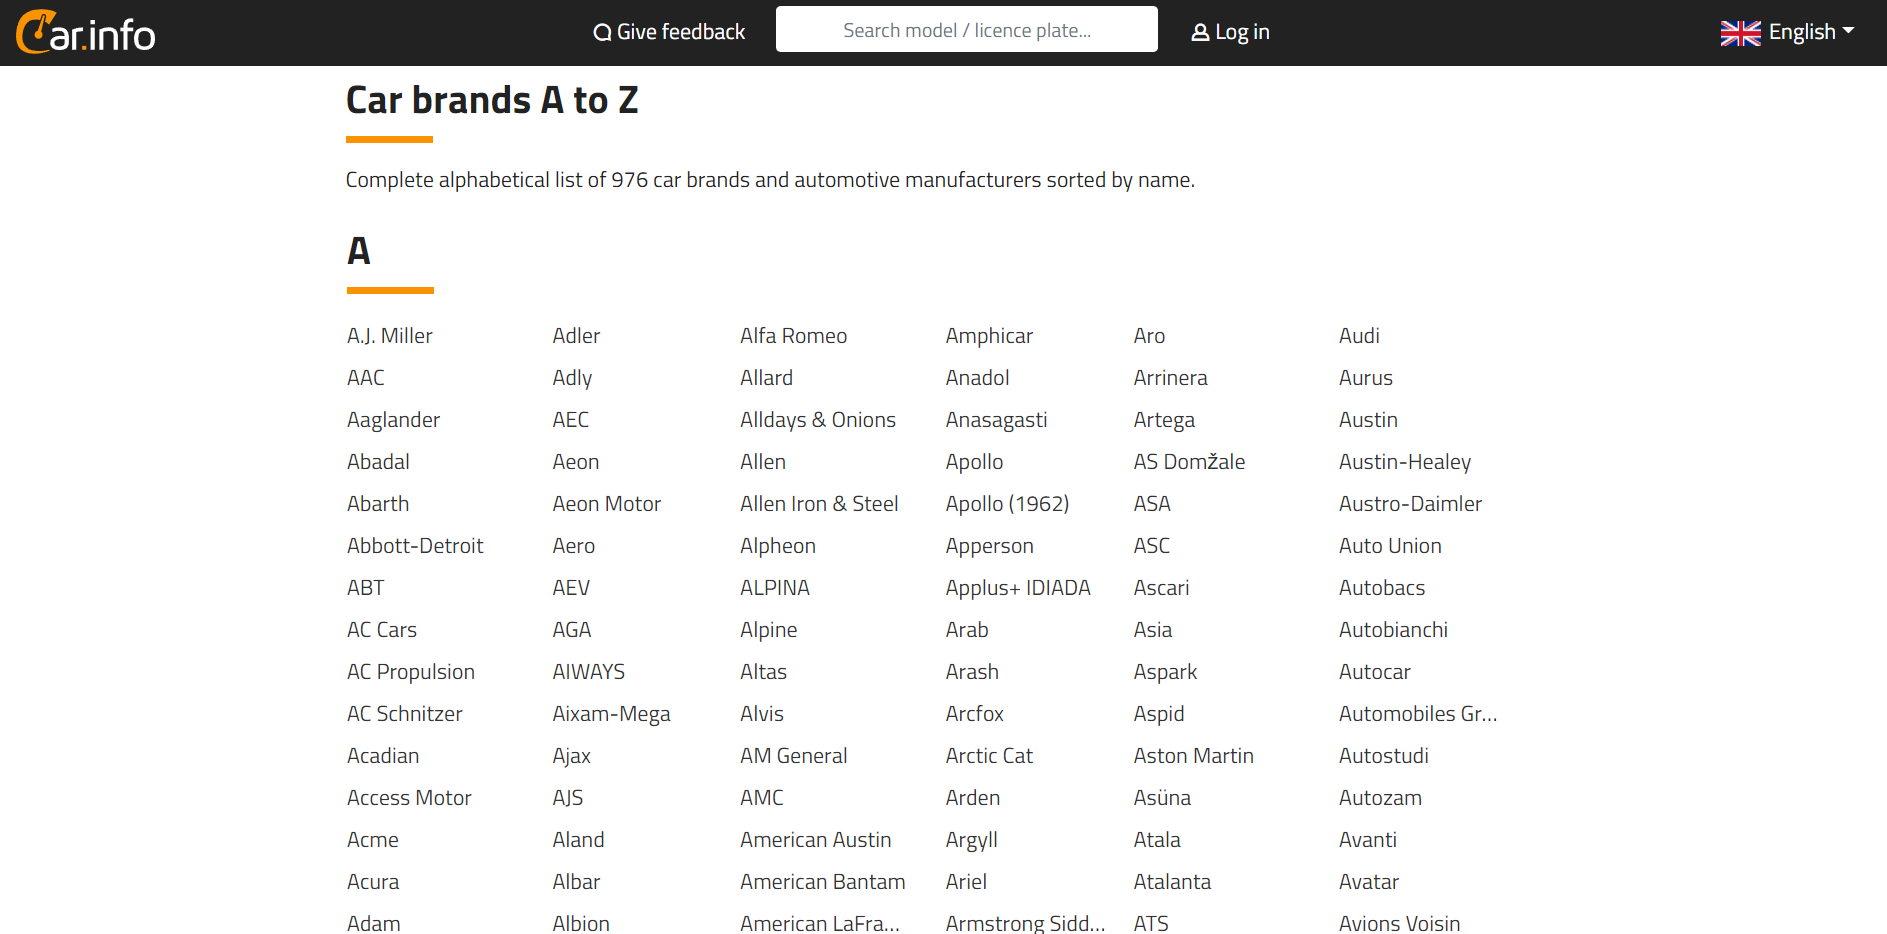
\includegraphics[width=\textwidth, height=\textheight, keepaspectratio]{car_info_brands_a_z}
	\caption{Car brands Catalogus van A tot Z op \url{https://www.car.info/en-se/brands}}
\end{figure}

Op het eerste zicht lijkt de webpagina reeds in een alfabetisch geordende tabelstructuur te staan. 
Het plan hierbij is om per element met de naam van het automerk een HTML attribuut te vinden die ieder HTML element die het automerk bevat deelt. Zo kan per tabelcel gezocht worden naar alle elementen die dit specifieke attribuut hebben.
We gebruiken Google Developer Tools om de HTML structuur van de webpagina te achterhalen.
\begin{figure}[H]
	\centering
	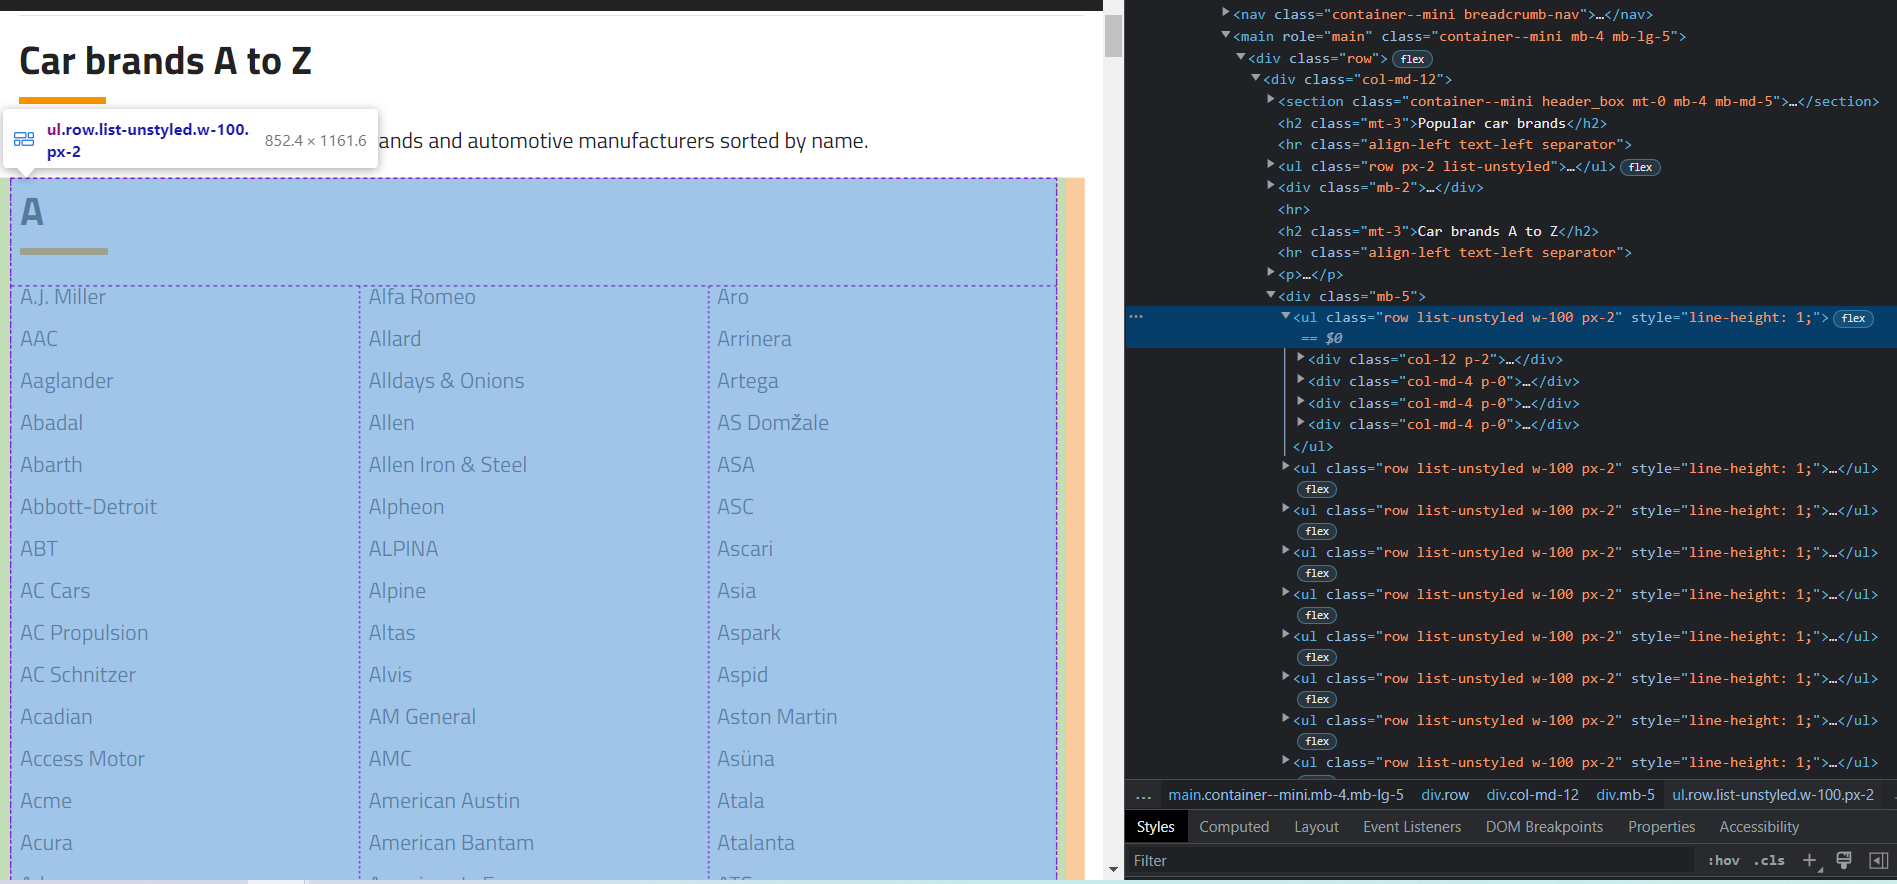
\includegraphics[width=\textwidth, height=\textheight, keepaspectratio]{car_info_a_z_html_outer_structure}
	\caption{Screenshot selecteren HTML element die alle automerken bevat}
\end{figure}
De ul tag met het class attribuut "row list-unstyled w-100 px-2" geeft ons de correcte selectors om deze elementen te vinden.
Dit element representeert een lijst met elementen in per specifieke letter in het alfabet. 
Er zal dus herhaaldelijk door dit soort elementen in een lus doorgegaan worden om voor iedere letter alle automerken te vinden.
Om dit te doen kijken we naar het element die alle ul elementen omvat, zijnde een div tag met class attribuut "mb-5".
De volgende stap is in deze elementen het tekstelement voor een automerk te achterhalen.
\begin{figure}[H]
	\centering
	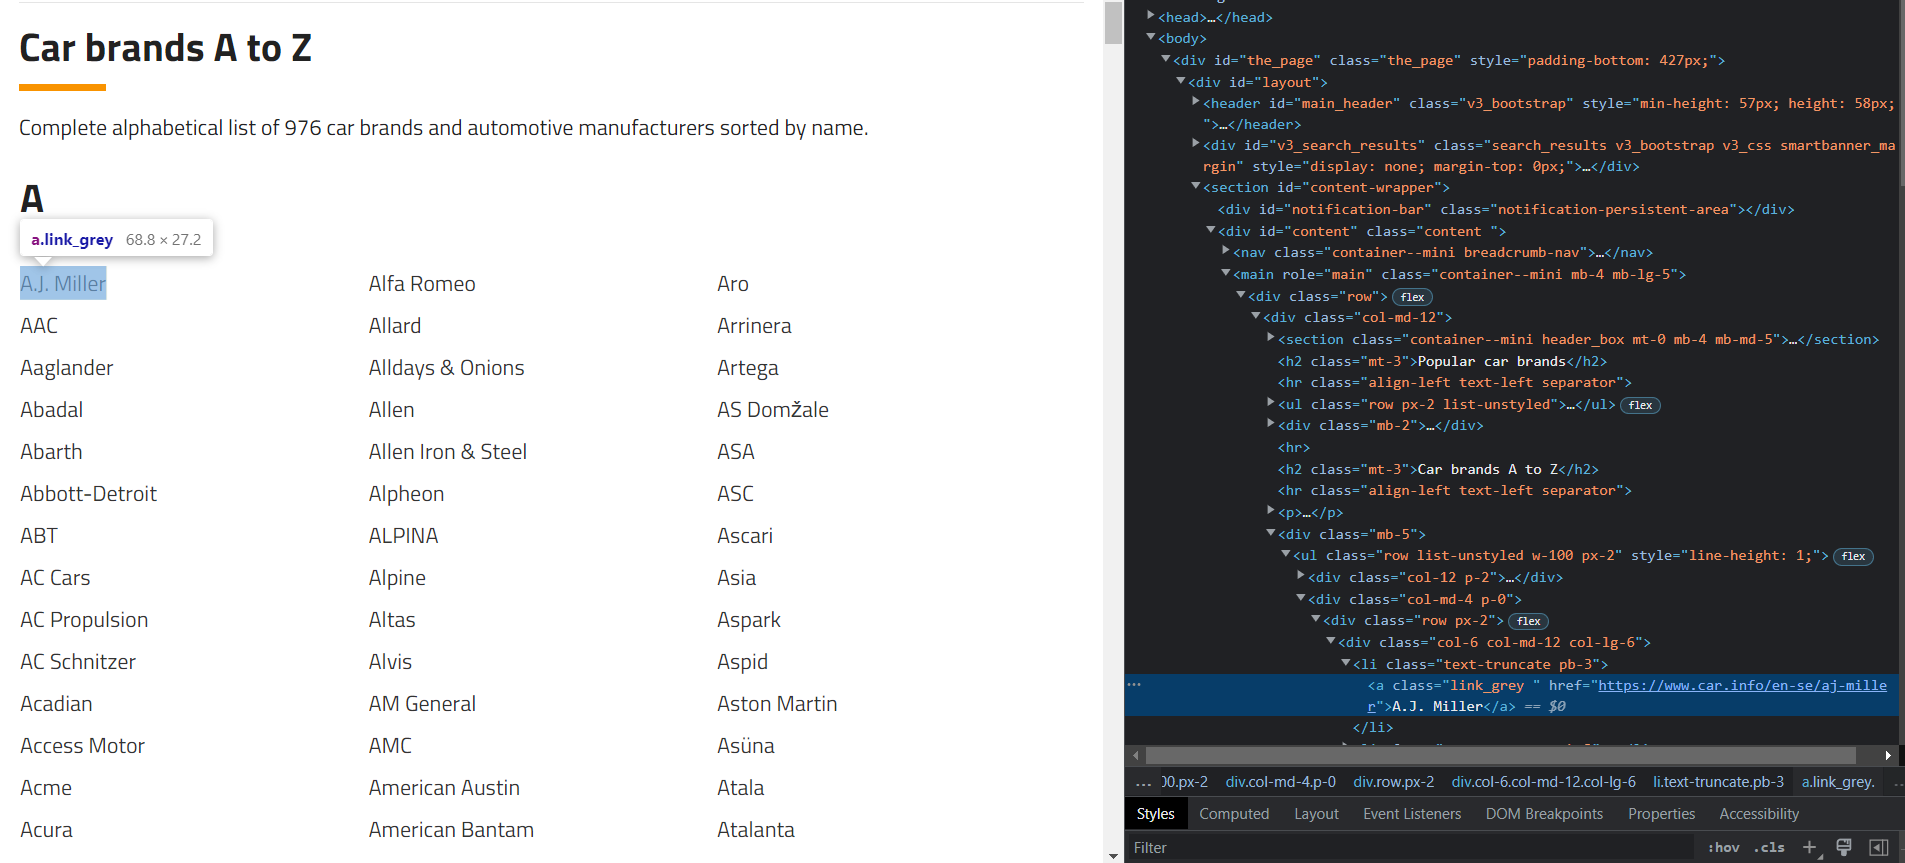
\includegraphics[width=\textwidth, height=\textheight, keepaspectratio]{car_info_a_z_html_car_brand_text}
	\caption{Screenshot selecteren HTML element die autotekst element bevat}
\end{figure}
De elementen in de ul tag die de tekst met het automerk beschrijven heeft overal eenzelfde structuur:
een a tag met als class "link\_grey". Van dit element wordt de tekst opgevraagd om enkele het automerk van dit element over te houden.
Zoals te zien is op de webpagina zijn de modellen per automerk niet zichtbaar op deze pagina. Hiervoor moet doorgeklikt worden naar de hyperlink die de tekst van het automerk bevat.
De waarde van het hyperlink attribuut wordt tijdelijk opgeslagen.
Opnieuw wordt de webscraper doorgestuurd naar een nieuwe webpagina met verschillende HTML elementen om de modellen te achterhalen. 

\begin{figure}[H]
	\centering
	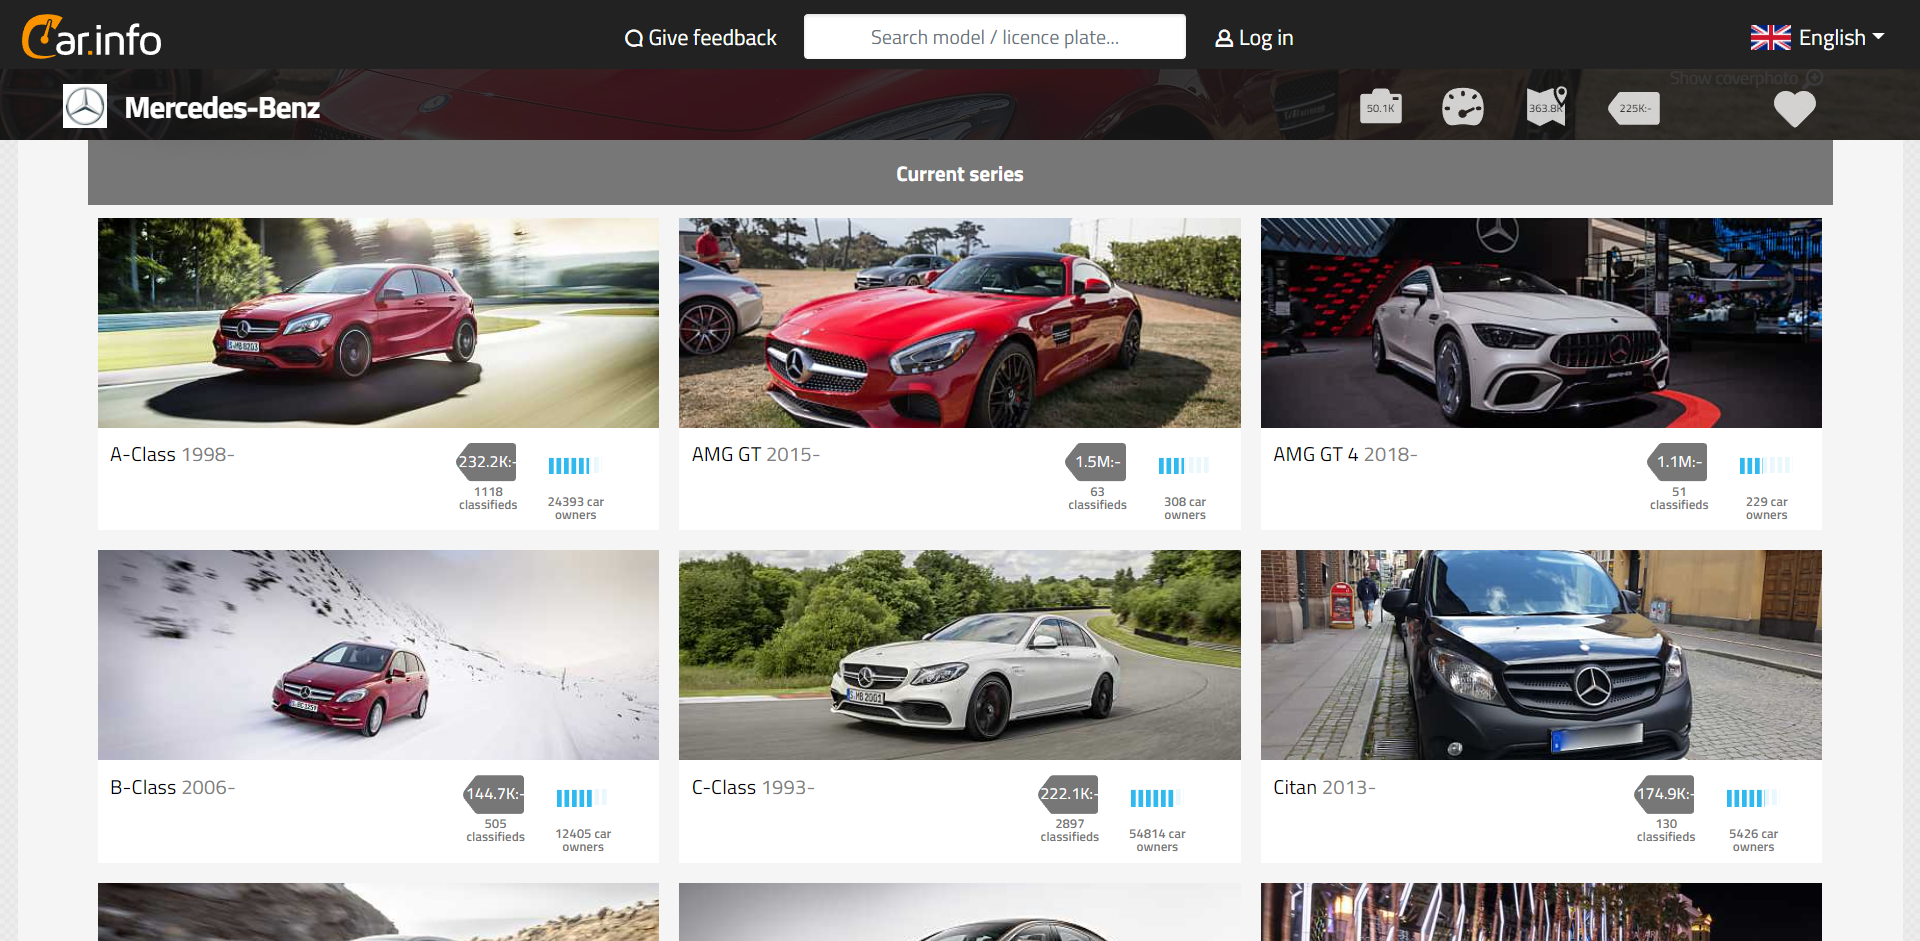
\includegraphics[width=\textwidth, height=\textheight, keepaspectratio]{car_info_mercedes_benz_modellen}
	\caption{Car info automodellen Mercedes-Benz op \url{https://www.car.info/en-se/mercedes-benz}}
\end{figure}

Deze webpagina toont alle modellen van een specifiek automerk, afhankelijk van welk merk, verschilt het aantal modellen. Hierin is de structuur anders dan de pagina voordien. De modellen zijn niet alfabetisch geordend maar eerder op serie of bouwjaar. Op deze webpagina wordt opnieuw gezocht naar het HTML element die de tekst met het model bevat en vervolgens wordt naar een gelijkenis gezocht in deze elementen om in een herhalende lus alle modellen uit de webpagina te halen.
We zien opnieuw in deze afbeelding dat ieder model eenzelfde stijl heeft: het automodel staat in het zwart en rechts ernaast staat in het lichtgrijs het bouwjaar.

\begin{figure}[H]
	\centering
	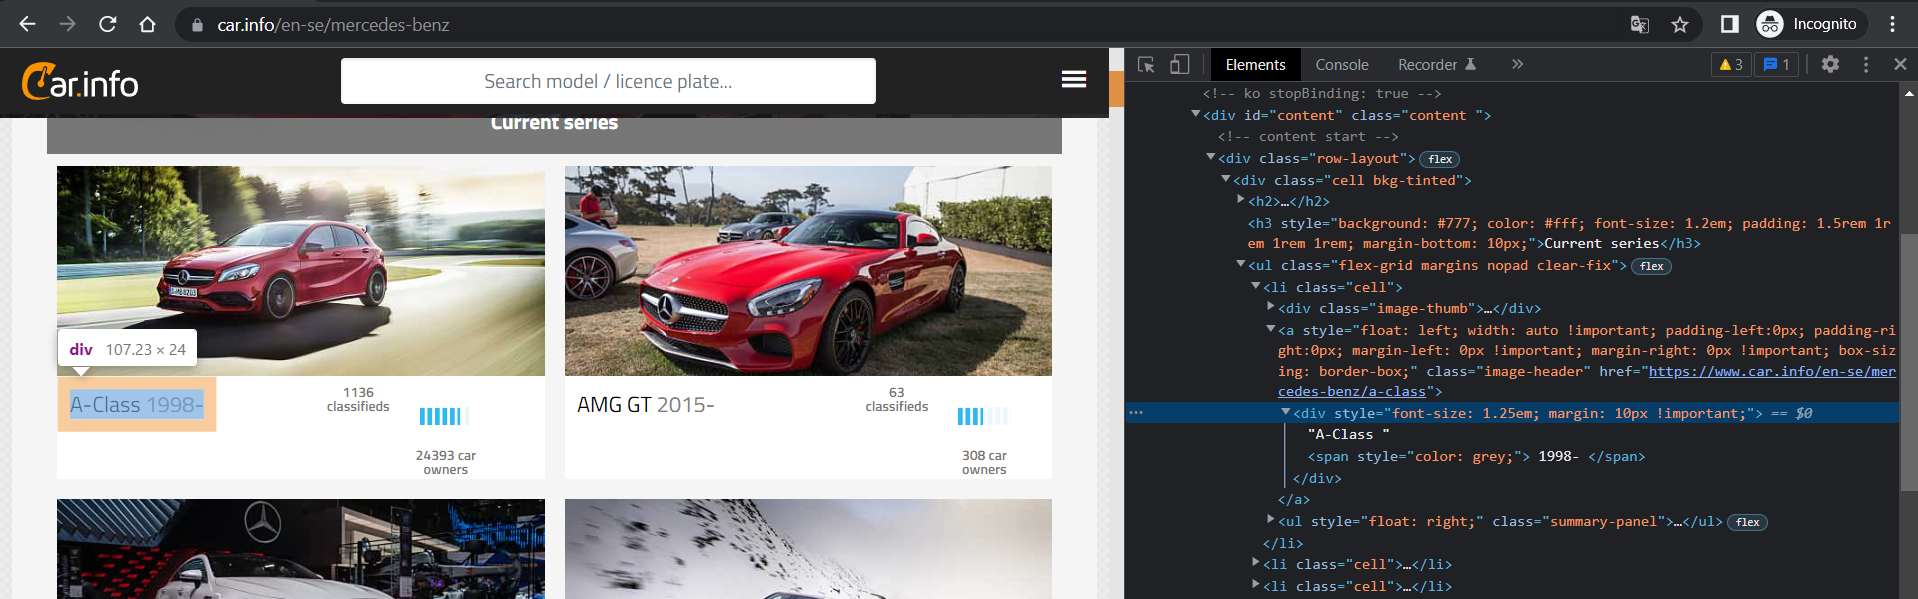
\includegraphics[width=\textwidth, height=\textheight, keepaspectratio]{car_info_specific_car_brand_html_car_model_text}
	\caption{Screenshot selecteren HTML element die het automodel en bouwjaar tekst bevat op car.info}
\end{figure}

Via Google Developer Tools achterhalen we dat al deze automodel elementen getypeerd worden door een div tag met daarin een style attribuut met als waarde "font-size: 1.25em; margin: 10px !important;" 
Eenmaal dit element achterhaald is, hoeft hier enkel de tekst uitgehaald te worden om zowel het automodel àls het bouwjaar op te slaan.
Als eindresultaat bekomen we per automerk een ongeordende lijst met alle modellen en hun bouwjaar. Dit is alles wat we nodig hebben om naar de volgende fase te gaan.

\subsubsection{Webscraping hindernissen}
Tijdens het onderzoek is het vooral van belang dat de data publiekelijk toegankelijk is om een databank of hun datastructuur op te zetten. Nu, niet iedere data is publiek en daar heeft de ontwikkelaar of het bedrijf op de webpagina zijn reden voor. Echter sommige data staat wel publiek, maar het is niet de bedoeling om deze te webscrapen. 
Onderstaande tabel lijst de meestvoorkomende obstructies op.
\begin{itemize}
	\item paywall of betalende service: 
	Hierbij is het eigenlijk enkel mogelijk om in te loggen of betalen voor de service voordat we eigenlijk toegang krijgt tot de data. De restrictie hier is dat hier een account of authenticatie aan gebonden is.
	\item dynamische html elementen:
	Voorgaande stand van zaken leert ons dat webpagina's of websscrapers gebruik maken van selectors om bepaalde elementen uit de webpagina te selecteren. 
	Nu doen web ontwikkelaars hun best soms op bepaalde pagina's om deze tags of attributen zo willekeurig mogelijk te maken. 
	Dit kan gebeuren door middel van bijvoorbeeld klasse attributen in elementen een willekeurige naam te geven iedere keer dat de pagina wordt ingeladen. 
	Zo krijgt webcrawler geen kans om telkens opnieuw hetzelfde klasse attribuut te gebruiken en verliest het zijn constentie.
	\item User agent:
	De User Agent houdt bij via welke browser een webpagina wordt bezocht.
	Een webontwikkelaar kan deze data uitlezen en kan nagaan via welke browser de de gebruiker de pagina bezoekt.
	Wanneer de webontwikkelaar ziet dat dit ongeldig is, zoals niet Google Chrome of een bestaande versie van, kan die de toegang voor die webpagina blokkeren.
	\item CAPTCHA:
	Een CAPTCHA is een antwoordtest die bij gegevensverwerking wordt gebruikt om na te gaan of er al dan niet een menselijke gebruiker is.
\end{itemize}
De exacte werking van enkele van de obstructies en hoe deze te omzeilen zijn wordt echter niet in dit onderzoek besproken.

\subsection{Data transformatie}
Om de data zo gestructureerd mogelijk te houden is er nood aan consistentie. Voornamelijk zien we al meteen dat bij automerken met verschillende woorden, zoals Range Rover, gebruik gemaakt wordt van hoofdletters. Om een probleem met inconsistente data te vermijden wordt hierbij alle data omgevormd naar drukletters. Bijvoorbeeld Mercedes-Benz wordt dus MERCEDES-BENZ. Aan de modellen is te zien dat er een bouwjaar op volgt. Dit werd in hetzelfde tekstelement genoteerd op de webpagina. Omdat deze extra info opgesplitst moet worden, zien we dat het bouwjaar altijd het laatste element is na de spatie. Door middel van op de laatste spatie te splitsen wordt nu een duidelijk onderscheid gemaakt tussen het model en het bouwjaar. Zo wordt “CLA 2013-“ omgevormd naar een lijst met ["CLA", "2013-"].

Dit kan in Python door middel van "slicing".

\begin{lstlisting}[language=Python, caption=Python splitst laatste element en alles ervoor op op spatie, breaklines=true, showstringspaces=false]
	car_model_buildyear = "CLA 2013-"
	car_model_buildyear_space_list = car_model_buildyear.split(" ") # ["CLA", "2013-"]
	car_model = " ".join(car_model_buildyear_space_list[:-1]) # "CLA"
	car_buildyear = car_model_buildyear_space_list[-1] # "2013-"
\end{lstlisting}

\subsection{Data opslaan}
Nu alle data in een correct formaat kan weergegeven worden, is het tijd om deze op te slaan in een databank. Omdat de data wordt opgehaald op basis van het automerk, en dit is ook de enige operatie is, hoeven er geen zware berekeningen of operaties via de databank of opslagstructuur gedaan te worden. Een key-value structuur is dus eigenlijk al genoeg zijn, de key zijnde het automerk, en het value een lijst met alle mogelijke modellen en hun desbetreffende bouwjaar voor dat automerk. Dit is mogelijk omdat het automerk een unieke waarde is waarop gefilterd kan worden.

\subsection{Programmatie}
Om alle bovenstaande informatie te verwerken via Selenium webscraper worden eerst en vooral alle relevante elementen opgeslagen.
Dit ziet er als volgt uit.
\begin{lstlisting}[language=Python, caption=Python houdt constanten bij van alle css selectors om elementen te vinden op de webpagina's, label={lst:selectors}, breaklines=true, showstringspaces=false]
# automerken selectors
car_brand_table_div_selector = "#content > main > div > div > div.mb-5"
car_brand_ul_alfabet_letter_selector = "ul"

# automodellen en bouwjaar selectors
car_model_buildyear_element_selector = "//div[@style='font-size: 1.25em; margin: 10px !important;']"
car_model_buildyear_text_selector = "link_grey"
\end{lstlisting}

Om een webpagina te bezoeken en te scrapen is er nood aan een instantie van een webscraper. Om te garanderen dat steeds de recentste Google Chrome versie wordt gebruikt, wordt gebruik gemaakt van de ChromeDriverManager, deze beheert het installatieproces van een Google Chrome Driver om bij Selenium webscraping te gebruiken. 
\begin{lstlisting}[language=Python, caption=Python declaratie en initialisatie Selenium webscraper, breaklines=true, showstringspaces=false]
	from selenium import webdriver
	from webdriver_manager.chrome import ChromeDriverManager
	from selenium.webdriver.chrome.service import Service
	
	driver = webdriver.Chrome(service=Service(ChromeDriverManager(log_level=0).install()))
\end{lstlisting}

Vervolgens wordt de webpagina bezocht en de vooraf element selectoren gebruikt om de elementen te vinden en op te halen.
\begin{lstlisting}[language=Python, caption=Selenium Webdriver haalt de webpagina op en vindt elementen, breaklines=true, showstringspaces=false]
	cars_catalogue_url = "https://www.car.info/en-se/brands"
	webdriver.get(cars_catalogue_url)
	div_element_table_with_all_carnames = webdriver.find_element(By.CSS_SELECTOR, selector_elements.car_brand_table_div_selector)
	unordered_list_per_alfabet_letter = div_element_table_with_all_carnames.find_elements(By.CSS_SELECTOR, selector_elements.car_brand_ul_alfabet_letter_selector)
\end{lstlisting}
De webdriver heeft een \texttt{find\_element} methode om elementen te zoeken op een webpagina. Het eerste argument is de CSS selector.
Nu de ongeordende lijst met elementen die per alfabetletter de automerken bevatten, wordt de extractie van ieder automerk met de link naar de modellen gecodeerd.
\begin{lstlisting}[language=Python, caption=Selenium Webdriver vindt per element het automerk en de link, breaklines=true, showstringspaces=false]
	car_url = "https://www.car.info/en-se/brands"
	webdriver.get(car_url)
	div_element_table_with_all_carnames = webdriver.find_element(By.CSS_SELECTOR, selector_elements.car_brand_table_div_selector)
	unordered_list_per_alfabet_letter = div_element_table_with_all_carnames.find_elements(By.CSS_SELECTOR, selector_elements.car_brand_ul_alfabet_letter_selector)
	
	list_carbrand_car_url_tuple = []  # voorbeeld [("Volvo", "www...",), ("Ferrari", "www...",)]
	for ul_alfabet_letter in unordered_list_per_alfabet_letter:
		alfabet_letter = ul_alfabet_letter.find_element(By.CSS_SELECTOR, "h2").text
		# slaat alle data op, startende met de alfabet letter
		carbrand_elements_for_current_letter = ul_alfabet_letter.find_elements(By.CLASS_NAME,
			selector_elements.car_model_buildyear_text_selector)
		for carbrand_element in carbrand_elements_for_current_letter:
			car_brand = carbrand_element.text
			car_brand_link = carbrand_element.get_attribute("href")
	# voeg automerk en autolink toe aan lijst
	list_carbrand_car_url_tuple.append((car_brand, car_brand_link,))
\end{lstlisting}
Nu ieder automerk tijdelijk is opgeslagen samen met bijhorende link naar de modellen, is het de bedoeling voor de webscraper om deze links te bezoeken en alle automodellen met het bouwjaar via de selector~\ref{lst:selectors} te vinden.
\begin{lstlisting}[language=Python, caption=Selenium Webdriver vindt automodellen en hun bouwjaar, breaklines=true, showstringspaces=false]
	# car_brand_link = om het even welke hyperlink naar een bestaand automerk waar de modellen zichtbaar zijn
	webdriver.get(car_brand_link)
	
	car_models_for_current_brand_elements = webdriver.find_elements(By.XPATH,
		selector_elements.car_model_buildyear_element_selector)
	
	# lijst opmaken
	car_model_data_list = [] # voorbeeld [{"modelnaam": "een_model", bouwjaar: "2000-2010"}, ...]}
	
	for car_model_with_buildyear_element in car_models_for_current_brand_elements:
		car_model_with_buildyear_split_by_spaces = car_model_with_buildyear_element.text.split(" ") # bijvoorbeeld ["A-Class", "1988-"]
		# als er een gekend bouwjaar staat in de lijst
		# autonaam wordt ook meteen IN HOOFDLETTERS geplaatst
		if len(car_model_with_buildyear_split_by_spaces) >= 2 and "-" in car_model_with_buildyear_split_by_spaces[-1]:
			car_model_name = " ".join(car_model_with_buildyear_split_by_spaces[:-1]).upper()
			car_model_buildyear = car_model_with_buildyear_split_by_spaces[-1]
		else:
			car_model_name = car_model_with_buildyear_split_by_spaces[0]
			car_model_buildyear = None
		
		#info aan lijst toevoegen
		# opnieuw data transformatie op het model
		car_model_info_structure = {"car_model": car_model_name.upper(), "car_buildyear": car_model_buildyear}
		car_model_data_list.append(car_model_info_structure)
\end{lstlisting}
Deze code wordt herhaald per automerk en kan dus uiteindelijk volgende structuur bekomen.
\begin{lstlisting}[language=json, caption=Eindresultaat formaat auto catalogus, label={formaat-auto-catalogus}, breaklines=true, showstringspaces=false]
	{"MERCEDES-BENZ": [
						{"car_model": "A-Class", "car_buildyear": "1998-"},
						{"car_model": "AMG GT", "car_buildyear": "2015-"},
						{...}
						],
	"BMW": [
			{"car_model": "1 Series", "car_buildyear": "2004-"},
			{...}
			],
	"...": [
			{...}
			]
	}
\end{lstlisting}

\subsection{Executie script}
De volledige code van dit script is toegankelijk op een \href{github repo}{https://github.com/GoddeerisEdouard/bachproef-latex/tree/main/prototype}
Tijdens het uitvoeren van dit script werd getimed hoelang dit duurt.
Volgens de specificaties van de gebruikte computer in dit onderzoek:
\begin{itemize}
	\item Computer model: Acer Aspire A715-74G
	\item CPU: Intel(R) Core(TM) i7-9750H CPU @ 2.60GHz   2.59 GHz
	\item RAM: 16,0 GB 
	\item OS / Besturingssysteem: Windows 10 Home
	\item Type systeem: 64-bits besturingssysteem, x64-processor
\end{itemize}
Met deze specificaties en verder geen andere programma's open duurde uitvoeren van het volledige script 14 minuten en 29 seconden.

\subsection{Data visualisatie}
Eenmaal de data is opgeslagen, kan deze gevisualiseerd worden om hier statistische informatie uit te halen. 
\begin{figure}[H]
	\centering
	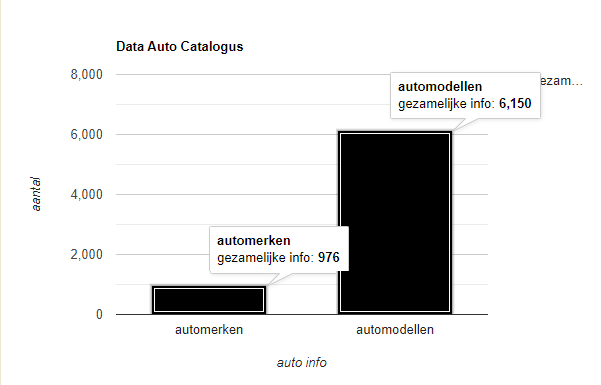
\includegraphics[width=\textwidth, height=\textheight, keepaspectratio]{aantal_autoinfo_waarden_bar_graph}
	\caption{Car info aantal waarden uit gescrapete data}
\end{figure}
De analyse van de visualisatie leert ons dat er \texttt{976} automerken in de auto catalogus zitten. Verder leert dit ons ook dat er \texttt{6150} automodellen zijn opgeslagen, die op hun beurt nog kunnen onderverdeeld worden in submodellen. Als laatste kan ook de gemiddelde lengte van alle automodellen worden berekend om de toetsslagen die bespaard worden te berekenen. Dit komt uit op een gemiddelde van \texttt{6} karakters per automodel.


\subsection{Implementatie}
Om de opgehaalde en gestructureerde data eenmaal te gaan gebruiken, is er nood aan een invulformulier waarin deze data kan gebruikt en verwerkt worden.
Met Python is het mogelijk in de console input van een gebruiker op te vragen en te verwerken.
Hiervoor kijkt men naar de stappen~\ref{sec:autoverzekering-stappen} die voordien werden uitgevoerd om de prijs van een autoverzekeringscontract te berekenen.
Via Python worden iteratief de velden die de klant moet invullen opgevraagd.
\begin{lstlisting}[language=Python, caption=Eerste velden autoverzekering digitaal invulformulier, breaklines=true, showstringspaces=false]
	voertuig_ouderdom = ""
	while voertuig_ouderdom not in ["y", "n"]:
		voertuig_ouderdom = input("Is uw voertuig ouder dan 2 jaar? (y/n) ")
	
	chassisnummer = input("Vul uw chassisnummer in, als u dit niet heeft, druk Enter ")
	if not chassisnummer:
		chassisnummer = -1
	print("Vul info over uw auto in:")
	brandstoftype = input("Brandstoftype: ")
	eerste_inschrijving = -1
	while 1800 > eerste_inschrijving or eerste_inschrijving > datetime.datetime.now().year:
		eerste_inschrijving = input("Eerste inschrijving: ")
		try:
			eerste_inschrijving = int(eerste_inschrijving)
		except ValueError:
			eerste_inschrijving = -1
			pass
\end{lstlisting}
Voor de eerste velden die ingevuld worden valt weinig te verbeteren, in het jaarveld wordt controle gedaan op een geldig inschrijvingsjaar, waarbij enkel logische jaartallen voor inschrijfdata worden toegelaten. 
\begin{lstlisting}[language=Python, caption=Python inladen data van auto catalogus, breaklines=true, showstringspaces=false]
	with open("car_data.json") as f:
		car_data = json.load(f)
	auto_model_keuzes = None
	while auto_model_keuzes is None:
		merk = input("Merk: ").upper()
		auto_model_keuzes = car_data.get(merk)
\end{lstlisting}
In dit deel van de code wordt de auto catalogus~\ref{formaat-auto-catalogus} ingeladen.
Meteen wordt ook dankzij de opgeslagen automerken herhaaldelijk gevraagd naar een bestaand automerk, zolang niet aan deze voorwaarde is voldaan zal blijvend aan de gebruiker gevraagd worden naar een bestaand automerk.
Nu komt het onderdeel waar de data die via de webscraper is opgehaald te pas komt.
Dankzij de modellen te hebben gecategoriseerd per automerk maakt dit het mogelijk voor de klant een selectie te maken tussen verschillende automodellen.
\begin{lstlisting}[language=Python, caption=Selenium Webdriver vindt automodellen en hun bouwjaar, breaklines=true, showstringspaces=false]
	print("Kies uw automodel:")
	# presenteert de automodellen in een genummerde lijst
	for teller, auto_model_keuze in enumerate(auto_model_keuzes):
		print(f"{teller + 1}. {auto_model_keuze['car_model']}")
	
	gekozen_auto_model = -1
	while not 0 <= gekozen_auto_model < len(auto_model_keuzes):
		gekozen_auto_model = input("keuze: ")
		try:
			gekozen_auto_model = int(gekozen_auto_model) - 1
		except ValueError:
			gekozen_auto_model = -1
		pass
	gekozen_auto_model_gevalideerd = auto_model_keuzes[gekozen_auto_model]
\end{lstlisting}
In dit onderdeel wordt gevraagd aan de gebruiker een selectie te maken tussen de verschillende bestaande automerken. Als het selectienummer niet in de lijst staat zal herhaaldelijk blijven gevraagd worden naar een bestaande getal binnen de opgegeven keuzes. Eenmaal een geldige keuze is opgegeven, wordt de bijhorende modeldata alsook het bouwjaar opgeslagen. 
Verder wordt aan de klant nog de cataloguswaarde van het voertuig gevraagd.
\begin{lstlisting}[language=Python, caption=Python code cataloguswaarde, breaklines=true, showstringspaces=false]
	cataloguswaarde = -1
	while cataloguswaarde <= 0:
		cataloguswaarde = input("Cataloguswaarde: ")
		try:
			cataloguswaarde = int(cataloguswaarde)
		except ValueError:
			cataloguswaarde = -1
			pass
\end{lstlisting}
Opnieuw wordt bij het laatste veld gecontroleerd als dit wel geldig is door te controleren als deze niet negatief of gratis is en wel degelijk een getal is.
Als laatste stap wordt al deze ingevoerde, geverifieerde en automatisch aangevulde data geformatteerd verwerkt.
\begin{figure}[H]
	\centering
	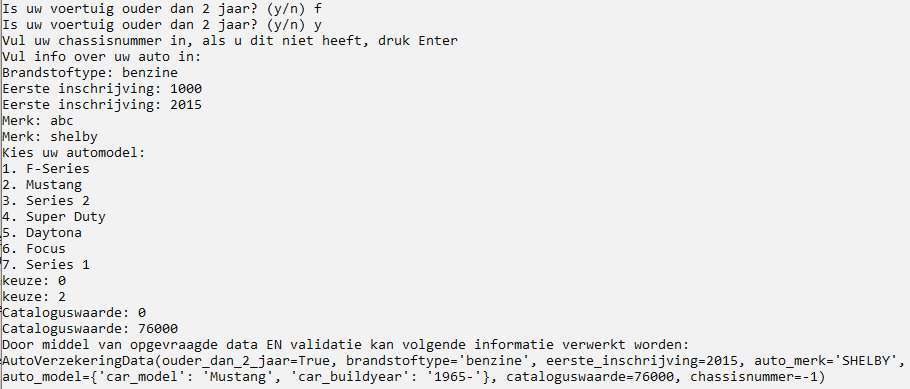
\includegraphics[width=\textwidth, height=\textheight, keepaspectratio]{python_auto_formulier_poc}
	\caption{Python digitaal autoverzekeringsformulier}
\end{figure}
In het uitgevoerde Python script wordt aangegeven dat de data gecontroleerd en verwerkt is en verder door een verzekeringsbedrijf kan geanalyseerd worden.


\subsection{Resultaten}
Wanneer de gegevens van voordien vergeleken worden met het digitale invulformulier waar gebruik werd gemaakt van datacontrole en geëxtraheerde data, vallen enkele zaken op. Uit de executie van het script om data op te halen lijkt dit een lang webscraping proces. Het is immers niet dagelijks of wekelijks nodig dit script uit te voeren, er komen namelijk niet dagelijks nieuwe automerken of automodellen op de markt. Het interval van het script is afhankelijk van welk soort data precies opgehaald moet worden en dus hoe dynamisch deze data is.
Er wordt een duidelijkheid onderscheid ondervonden in het aantal in te vullen velden via een digitaal formulier tegenover een manueel document. De velden~\ref{enum:autoverzekering-stappen} die voordien door de klant moesten ingevuld worden zijn hierbij gereduceerd.
Er valt duidelijk te zien dat dankzij dit digitaal formulier een aantal factoren die voor verwarring of ongeldigheid zouden kunnen zorgen bij ontvangst van het verzekeringskantoor worden geëlimineerd.
Zo is er strikte validatie op de velden, en niet alleen op velden die vrij in te vullen zijn door de eindgebruiker.
Zo worden ook bepaalde velden automatisch ingevuld, of wordt er een selectie aan mogelijke antwoorden gepresenteerd.
Het verschil in in te vullen lijkt op het eerste zicht niet veel, maar op een klein formulier is dit toch een verbetering van 12,5\% (1 van de 8 velden verdwijnt). Laten we voorstellen dat het invulformulier meer data, verwant met het model zou vragen zou dit percentage alleen maar accumuleren.
In principe zou de cataloguswaarde van dit model ook kunnen opgehaald worden, wat het optimalisatiepercentage alleen maar verhoogt (25\%).
